\documentclass[9pt]{beamer}
\beamertemplatenavigationsymbolsempty

\usepackage[T1]{fontenc}
\usepackage{subfig}
%\usetheme{Berlin}

\definecolor{TriangleColor}{RGB}{255,170,128} % Soft Coral
\definecolor{LineColor}{RGB}{0,128,128} % Darker Blue
\definecolor{VertexColor}{RGB}{255,255,128} % Light Yellow


\usepackage{etex, tikz, array, graphics, xspace, relsize, multirow}
\usepackage[export]{adjustbox}
\usepackage{ulem}
\usepackage{faktor}

\usetikzlibrary{arrows}
\usetikzlibrary{tikzmark}
\input binhex

\makeatletter
\PassOptionsToPackage{sortcites,isbn=false}{biblatex}


% Set frame title color
\setbeamercolor{frametitle}{fg=LineColor}

% Set section title color
\setbeamercolor{title}{fg=LineColor}



\renewenvironment{theorem}[1][]
{\textcolor{LineColor}{\textbf{Theorem #1}} }
{}

\renewenvironment{definition}[1][]
{\textcolor{LineColor}{\textbf{Definition #1}} }
{}

\renewenvironment{problem}[1][]
{\textcolor{LineColor}{\textbf{Problem #1}} }
{}

\renewenvironment{lemma}[1][]
{\textcolor{LineColor}{\textbf{Lemma #1 }} }
{}

% Set subtitle color
\setbeamercolor{subtitle}{fg=LineColor}

\usepackage{enumitem}
\setlist[itemize]{label=\textcolor{LineColor}{\textbullet}}
\PassOptionsToPackage{hyperfootnotes=false}{hyperref}
\PassOptionsToPackage{capitalise}{cleveref}
\usepackage{bbding}
\usepackage{pdflscape}
\usepackage{rotating}\setlength{\rotFPtop}{0pt plus 1fil}
\usepackage{layout}
\overfullrule=1ex


\usepackage[textsize=tiny]{todonotes}
\setlength{\marginparwidth}{1.75cm}
\setlength{\marginparsep}{1mm}


% Data tables
\usepackage{siunitx}
\sisetup{reset-math-version = false}
\sisetup{table-auto-round}
\usepackage{xstring}

\usepackage[legacy]{csvsimple}

\sisetup{reset-math-version = false}
\sisetup{table-auto-round}

% For code inclusion
\usepackage{listings}
\lstset{ breaklines=true}
\lstset{escapeinside={<@}{@>}}
\usepackage{algorithm,algorithmic}

\renewcommand{\algorithmicrequire}{\textbf{Input:}}
\renewcommand{\algorithmicensure}{\textbf{Output:}}



\usepackage{svg}
\usepackage{nicematrix}

\usepackage[legacy]{csvsimple}

% For drawing
%% Tikz drawing
\usepackage{tikz} \usetikzlibrary{arrows} \usetikzlibrary{arrows.meta}
\usepackage{pgfplots} \usepackage{tikz-3dplot} \usepackage{tcolorbox}
\usetikzlibrary{matrix,fit,positioning,shapes.geometric,patterns,backgrounds}
\usetikzlibrary{decorations.pathreplacing}
\usetikzlibrary{decorations.markings} \usetikzlibrary{arrows,calc}
\tikzstyle{bigbox} = [draw=blue!50, thick, rounded corners, rectangle]
\tikzset{ >=stealth' } \tikzset{->-/.style={decoration={ markings,
      mark=at position #1 with {\arrow{>}}},postaction={decorate}}}


\usepackage{tikz}
\usetikzlibrary{positioning}
\usepackage[draft=false]{minted}
\usemintedstyle{default}
\setminted{fontsize=\footnotesize, frame=single, framesep=2mm}

\newcommand\Julia{\texttt{Julia}\xspace}
\newcommand\OSCAR{\texttt{OSCAR}\xspace}
\newcommand\Macaulay{\texttt{Macaulay2}\xspace}
\newcommand\Magma{\texttt{Magma}\xspace}
\newcommand\Sage{\texttt{SageMath}\xspace}
\newcommand\ZZ{{\mathbb Z}}
\newcommand\QQ{{\mathbb Q}}
\newcommand\PP{{\mathbb P}}

\usepackage{xcolor}
\definecolor{green}{rgb}{0.1,0.59,0.1}
\definecolor{yellow}{rgb}{0.8,0.67,0}
\definecolor{red}{rgb}{0.89,0.1,0.1}
\definecolor{blue}{rgb}{0.1,0.1,0.89}

\usenavigationsymbolstemplate{}

\usepackage{booktabs}
% For software citations
\newcommand{\singular}{\texttt{Sin\-gu\-lar}\xspace}
\newcommand\CPP{C\nolinebreak\hspace{-.05em}\raisebox{.4ex}{\relsize{-3}{\textbf{+}}}\nolinebreak\hspace{-.10em}\raisebox{.4ex}{\relsize{-3}{\textbf{+}}}\xspace}

\usepackage{amsmath}
\newcommand{\mrdi}{\texttt{mrdi}\xspace}

\newcommand{\pmsmall}{
\includegraphics[scale=0.03]{pmlogo.png}}
\newcommand{\pmlogo}{
\includegraphics[scale=0.09]{pmlogo.png}}
\newcommand{\pmbluesmall}{\includegraphics[scale=0.03]{pmbluelogo.png}}
\newcommand{\Disjoint}{\mathop{\coprod}}
\newcommand{\Discriminant}{\mathcal{D}}

\author[Antony Della Vecchia]{Antony Della Vecchia}
\title{Serializing Algebraic Data}

\institute[]{
  TU Berlin
}
\date{
  JuliaCon 2026-08-12
}

\newcommand{\surj}{\twoheadrightarrow}
\newcommand{\oursetting}[1]{\textcolor{blue}{#1}}

% Itemize that spreads its items to fill the frame vertically
\newenvironment{fillitemize}
  {\vspace{\fill}\begin{itemize}\setlength{\itemsep}{\fill}}
  {\end{itemize}\vspace{\fill}}

% Worker-pool star graph, reused on the title page and the multiprocessing slide
\newcommand{\workerpoolgraph}[1][0.55]{%
  \begin{tikzpicture}[scale=#1, every node/.append style={transform shape},
    main/.style={circle, draw=LineColor, thick, fill=TriangleColor, minimum size=2.0cm, align=center, font=\small\bfseries},
    worker/.style={circle, draw=LineColor, thick, fill=VertexColor, minimum size=1.0cm, align=center, font=\small},
  ]
    \node[main] (center) {Main};
    \node[worker, above=1.3cm of center]       (p1) {P1};
    \node[worker, above right=1.0cm and 1.3cm of center] (p2) {P2};
    \node[worker, right=1.7cm of center]         (p3) {P3};
    \node[worker, below right=1.0cm and 1.3cm of center] (p4) {P4};
    \node[worker, below=1.3cm of center]       (p5) {P5};
    \node[worker, below left=1.0cm and 1.3cm of center]  (p6) {P6};
    \node[worker, left=1.7cm of center]          (p7) {P7};
    \node[worker, above left=1.0cm and 1.3cm of center]  (p8) {P8};
    \foreach \p in {p1,p2,p3,p4,p5,p6,p7,p8} \draw[<->, LineColor, thick] (center) -- (\p);
  \end{tikzpicture}%
}

\begin{document}

% Left-aligned title page with the mrdi tree diagram
\begin{frame}[plain]
  \vfill
  \begin{columns}[c]
    \begin{column}{0.5\textwidth}
      \raggedright
      {\usebeamercolor[fg]{title}\usebeamerfont{title}\inserttitle\par}
      \bigskip

      {\usebeamerfont{author}\insertauthor\par}
      \medskip

      {\usebeamercolor[fg]{institute}\usebeamerfont{institute}\insertinstitute\par}
      \smallskip

      {\usebeamerfont{date}\insertdate\par}

    \end{column}
    \begin{column}{0.5\textwidth}
      \centering
      
\includegraphics[width=0.75\textwidth]{images/tree-coloured}
    \end{column}
  \end{columns}
  \vfill
  \noindent
  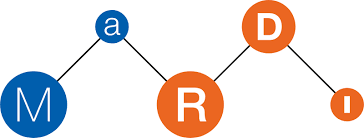
\includegraphics[width=2.2cm]{images/mardi-logo.png}%
  \hfill
  
\includegraphics[width=2.2cm]{images/oscar.pdf}

\end{frame}

%% Slide 1 --- Motivation
\begin{frame}{Serializing Algebraic Data}
  \textbf{Serialization:} translate in-memory data to a form that can be
  \emph{stored} or \emph{transmitted}, then reconstructed on another process
  or machine.
  \bigskip
  \bigskip

  Say we want to store:
  \begin{align*}
    p = 2y^3z^4 + (\mathbf{a} + 3)z^2 + 5\mathbf{a}y + 1
  \end{align*}
  \pause
  \begin{itemize}
  \item Is $y$ considered a coefficient of $z$?
  \item What is $\mathbf{a}$? \pause
  \item How can we guarantee the objects behave as expected on load? \pause
  \item Elements sharing a parent should have the same parent on load.
  \end{itemize}
\end{frame}

\begin{frame}[fragile]{The \mrdi File Format}
  \begin{columns}[T]
    \begin{column}{0.42\textwidth}
      \centering
      
\includegraphics[width=\textwidth]{images/tree-coloured}
    \end{column}
    \begin{column}{0.58\textwidth}
      \vspace{4mm}
      \pause
      \begin{itemize}
      \item ICMS 2024 [DV - Joswig - Lorenz].
        \vspace{2mm}
      \item Initial focus on long term storage.
        \vspace{2mm}
      \item JSON based.
        \vspace{2mm}
      \item \texttt{\_ns} pins semantics.
        \vspace{2mm}
      \item \texttt{\_type} subtree describes the data and it's algebraic context.
        \vspace{2mm}
      \item Shared parents (e.g. the ring) stored once in \texttt{\_refs},
        addressed by UUID.
        \vspace{2mm}
      \item Implementations for \Macaulay (Doug Torrance), \Magma(Jeroen Hanselman) and \Sage
      \end{itemize}
    \end{column}
  \end{columns}
\end{frame}

%% Slide 3 --- Adding serialization support for a new type
\begin{frame}[fragile]{Serialization Framework}
  Adding support for a new type means implementing three functions.
  \vspace{3mm}
  \begin{tcolorbox}[colframe=LineColor, colback=white, boxrule=0.5pt]
    \begin{itemize}\itemsep=\smallskipamount
    \item \texttt{type\_and\_params} --- returns the context needed to
      rebuild the object (e.g.\ its parent ring).
      \vspace{3mm}
    \item \texttt{save\_object} --- writes the \texttt{data} subtree.
      \vspace{3mm}
    \item \texttt{load\_object} --- reads the \texttt{data} subtree expects context to be provided.
    \end{itemize}
  \end{tcolorbox}
  \pause
  \vspace{3mm}
  \begin{tcolorbox}[colframe=LineColor, colback=white, boxrule=0.5pt]
    \begin{itemize}\itemsep=\smallskipamount
    \item General framework handles container types.
      \vspace{3mm}
    \item Entire sessions can be stored across multiple files.
      \vspace{3mm}
    \item Coercion --- loading files into a given algebraic context.
    \end{itemize}
  \end{tcolorbox}
\end{frame}


%% Slide 5 --- Serializers: multiple dispatch on encoding
\begin{frame}[fragile]{Serializers}
  \inputminted{jl}{oscar-snippet}
  \footnotesize
  \bigskip
  \pause
  \begin{columns}[T]
    \begin{column}{0.42\textwidth}
      \centering
      
\includegraphics[width=0.9\textwidth]{images/tree-dense}
    \end{column}
    \begin{column}{0.58\textwidth}
      \begin{itemize}\itemsep=\smallskipamount
      \item Selection of different serializers lets users alter subtrees.
        \vspace{2mm}
      \item Parametrized \texttt{SerializerState\{S\}}
        \vspace{2mm}
      \item Multiple dispatch on \texttt{S} selects the encoding per context 
        \vspace{2mm}
      \item Currently available: \texttt{JSONSerializer}, \texttt{IPCSerializer},
        \texttt{LPSerializer}, \texttt{MultiFileRef}.
      \end{itemize}
    \end{column}
  \end{columns}
\end{frame}

%% Slide 4 --- Multiprocessing (single slide)
\begin{frame}{Multiprocessing}
  \begin{columns}[T]
    \begin{column}{0.42\textwidth}
      \begin{center}
        \workerpoolgraph[0.55]
      \end{center}
    \end{column}
    \begin{column}{0.58\textwidth}
      \textbf{\texttt{OscarWorkerPool}} --- subtype of \Julia's
      \texttt{AbstractWorkerPool}, Uses the \texttt{IPCserializer}.
      \begin{itemize}
      \item Sends context to workers once, then reuses an
        \texttt{IPCSerializer} for every message.
      \item \Julia's \texttt{remotecall} and \texttt{pmap} work directly with
        \OSCAR types.
      \item Works with cluster managers (\texttt{SlurmClusterManager.jl})
      \item \textbf{32 processes, \SI{150}{\giga\byte}: $<3$ hours vs.\
        $>24$ hours (1 process)} found degree-5 components of vanishing-ideal for $\sigma_4(\PP^3 \times \PP^3 \times \PP^3).
      \end{itemize}
    \end{column}
  \end{columns}
\end{frame}

%% Slide 6 --- Future work
\begin{frame}[fragile]{Future Work}
  \begin{itemize}\itemsep=\smallskipamount
  \item Spin off the serialization code into a standalone \Julia package.
    \vspace{3mm}
  \item Add support for binary formats.
    \vspace{3mm}
  \end{itemize}
  \vfill
  \pause
  \begin{center}
    \Large Thank You!
  \end{center}
\end{frame}

\end{document}
